% Standalone Beamer revision of Class 16.
% Optional original plots: place images/class16_*.pdf next to this file.
\documentclass[aspectratio=169,11pt]{beamer}
\usepackage[T1]{fontenc}
\usepackage[utf8]{inputenc}
\usepackage{lmodern,amsmath,amssymb,booktabs,tabularx,array,graphicx,tikz,xcolor}
\usetikzlibrary{positioning,arrows.meta,shapes.geometric}
\definecolor{courseblue}{HTML}{183F67}
\definecolor{coursegold}{HTML}{C88A2B}
\definecolor{courseice}{HTML}{EEF4F8}
\definecolor{coursegray}{HTML}{66727B}
\setbeamercolor{structure}{fg=courseblue}
\setbeamercolor{frametitle}{fg=courseblue,bg=courseice}
\setbeamercolor{block title}{fg=white,bg=courseblue}
\setbeamercolor{block body}{fg=black,bg=courseice}
\setbeamertemplate{navigation symbols}{}
\setbeamertemplate{itemize item}{\color{coursegold}$\bullet$}
\setbeamertemplate{footline}{\hspace{0.5em}\scriptsize University of Trieste\hfill Data-driven Systems Engineering $\mid$ 440MI / 305SM\hfill \insertframenumber/\inserttotalframenumber\hspace{0.8em}\vspace{0.3em}}
\newcommand{\coursename}{Data-driven Systems Engineering}
\newcommand{\coursefooter}{}
\newcommand{\repoactivity}[1]{\begin{block}{Repository activity}#1\end{block}}
\newcommand{\readinglist}[1]{\begin{block}{Papers and materials}#1\end{block}}
\tikzset{flowbox/.style={draw=courseblue,fill=courseice,rounded corners=2pt,align=center},
accentbox/.style={draw=coursegold,fill=coursegold!12,rounded corners=2pt,align=center},
arrow/.style={-Latex,thick,draw=courseblue}}
% Preserves references to original illustrations without preventing compilation
% when only the .tex file is available.
\newcommand{\optionalfigure}[2]{%
\IfFileExists{#1}{\includegraphics[#2]{#1}}{%
\fcolorbox{courseblue}{courseice}{\parbox[c][3.0cm][c]{0.82\linewidth}{\centering\footnotesize Original figure not bundled\\[0.4em]\texttt{\detokenize{#1}}\\[0.4em]Copy the original images/ folder here.}}}}


\title{Class 16: Feature Engineering --- From Raw Data to Validated Features}
\author{\coursename}
\date{}

\begin{document}

\frame{\titlepage \coursefooter}

\begin{frame}{Agenda}
\begin{itemize}
\item Why feature engineering remains necessary once every variable is numerically encoded.
\item Data curation throughout the workflow: documentation, versioning, and validation.
\item Data cleaning: missing values, duplicates, invalid values, and outliers.
\item Feature construction from domain knowledge, for tabular data and data streams.
\item Feature representation before selection: encoding, scaling, and PCA (Class 14).
\item Feature selection: filter, wrapper, and embedded methods.
\item Leakage and availability checks before deployment.
\item Titanic running case: baseline, ablation, evaluation, and reproducible pipeline.
\end{itemize}
\coursefooter
\end{frame}
\begin{frame}{Why feature engineering remains necessary after encoding}
\begin{itemize}
\item Class 14 explained numerical representations; this class places them in a workflow. Encoding alone does not make a variable correct, reliable, or informative.
\item Real datasets contain missing values, duplicates, and inconsistent types, which must be resolved before an encoding is meaningful.
\item Not every available variable should become a feature: some are redundant, some carry only noise, and some induce leakage.
\item Informative features are frequently absent from the raw data and must be constructed from domain knowledge.
\end{itemize}
\coursefooter
\end{frame}
\begin{frame}{Feature engineering in the modeling workflow}
\centering
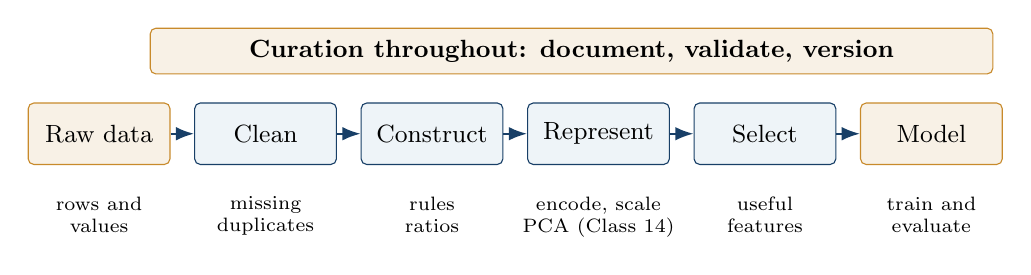
\begin{tikzpicture}[node distance=0.3cm]
\node[accentbox, minimum width=1.8cm, minimum height=0.78cm, font=\small] (raw) {Raw data};
\node[flowbox, minimum width=1.8cm, minimum height=0.78cm, font=\small, right=of raw] (clean) {Clean};
\node[flowbox, minimum width=1.8cm, minimum height=0.78cm, font=\small, right=of clean] (construct) {Construct};
\node[flowbox, minimum width=1.8cm, minimum height=0.78cm, font=\small, right=of construct] (encode) {Represent};
\node[flowbox, minimum width=1.8cm, minimum height=0.78cm, font=\small, right=of encode] (select) {Select};
\node[accentbox, minimum width=1.8cm, minimum height=0.78cm, font=\small, right=of select] (model) {Model};
\draw[arrow] (raw) -- (clean);
\draw[arrow] (clean) -- (construct);
\draw[arrow] (construct) -- (encode);
\draw[arrow] (encode) -- (select);
\draw[arrow] (select) -- (model);
\node[below=0.28cm of raw, font=\scriptsize, align=center] {rows and\\values};
\node[below=0.28cm of clean, font=\scriptsize, align=center] {missing\\duplicates};
\node[below=0.28cm of construct, font=\scriptsize, align=center] {rules\\ratios};
\node[below=0.28cm of encode, font=\scriptsize, align=center] {encode, scale\\PCA (Class 14)};
\node[below=0.28cm of select, font=\scriptsize, align=center] {useful\\features};
\node[below=0.28cm of model, font=\scriptsize, align=center] {train and\\evaluate};
\node[accentbox, minimum width=10.7cm, minimum height=0.58cm, font=\small\bfseries] at (6.0,1.05) {Curation throughout: document, validate, version};
\end{tikzpicture}

\vspace{0.25em}
\begin{block}{Feature construction and transformation}
\centering\small
Construction creates candidate features (e.g., ratios or rolling means). It is one kind of feature transformation; encoding and scaling also transform features, while selection chooses which candidates to keep.
\end{block}
\vspace{-0.25em}
{\scriptsize The workflow is iterative: reject leaking or unavailable features early; construction and selection may be revisited. PCA constructs components rather than selecting original columns.}
\coursefooter
\end{frame}
\begin{frame}{Running case: Titanic survival prediction}
\begin{block}{Engineering question}
Can we predict whether a passenger survives, using only information available at the intended prediction moment?
\end{block}
\begin{columns}[T]
\column{0.52\textwidth}
\begin{itemize}\small
\item \textbf{Target:} \texttt{survived} (binary), $n=891$ passengers.
\item \textbf{Raw candidates:} \texttt{age}, \texttt{sex}, \texttt{pclass}, \texttt{fare}, \texttt{sibsp}, \texttt{parch}, \texttt{embarked}.
\item \textbf{Suspicious candidates:} \texttt{alive} and any attribute defined using outcomes after the event.
\end{itemize}
\column{0.46\textwidth}
\begin{block}{Evidence we will reveal}\small
Raw $\rightarrow$ Curate $\rightarrow$ Clean $\rightarrow$ Construct $\rightarrow$ Represent $\rightarrow$ Select $\rightarrow$ Validate.
\end{block}
\end{columns}
\vspace{0.3em}
\textbf{Class discussion:} Is a variable useful just because it is predictive?
\coursefooter
\end{frame}
\begin{frame}{Data curation}
\begin{itemize}
\item Curation makes a dataset understandable and reusable beyond its original authors.
\item A data dictionary records the meaning, unit, and valid range of every column.
\item Capture provenance and lineage: source, extraction/query, timestamp, version, and feature definitions; an extraction date alone does not guarantee reproducibility.
\item Validation rules (schema and range checks) detect upstream problems before they reach the modeling stage.
\end{itemize}
\begin{block}{Repository example}
For Titanic, record a feature contract: definition, type, allowed values, missingness policy, source, prediction-time availability, and version. The fraud-case specification in \texttt{documents/FraudDetectionAsaService.pdf} illustrates similar documentation.
\end{block}
\coursefooter
\end{frame}
\begin{frame}{Titanic / 1: curate the feature contract}
\small
\begin{tabularx}{\textwidth}{>{\ttfamily}l l X X}
\normalfont\bfseries Field & \bfseries Type & \bfseries Meaning / validation & \bfseries Prediction-time audit \\
\toprule
survived & binary & Target; 0 or 1 & Never an input \\
sex & nominal & Passenger category & Check available \\
age & numeric & Age in years; missing possible & Check available \\
sibsp & count & Siblings/spouses aboard; $\ge 0$ & Check available \\
parch & count & Parents/children aboard; $\ge 0$ & Check available \\
embarked & nominal & Embarkation port; some missing & Check available \\
alive & nominal & Outcome-derived survival label & \textcolor{red}{Exclude: target leakage} \\
\bottomrule
\end{tabularx}
\vspace{0.5em}
\begin{block}{What should be versioned?}
\small Dataset snapshot / extraction, column schema, validation rules, cleaning and construction code, split definition, and fitted preprocessing artifacts.
\end{block}
\textbf{Question:} Which fields would you reject \emph{before} looking at feature scores?
\coursefooter
\end{frame}
\begin{frame}{Data cleaning: scope and quality dimensions}
\centering
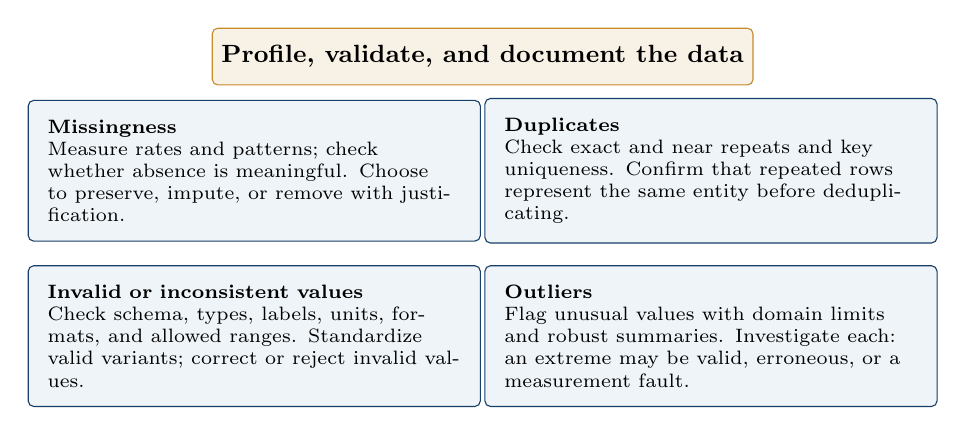
\begin{tikzpicture}
\node[accentbox, minimum width=6.6cm, minimum height=0.72cm, font=\small\bfseries] at (0,0) {Profile, validate, and document the data};
\node[flowbox, text width=5.25cm, minimum height=1.45cm, align=left, inner sep=7pt, font=\scriptsize] at (-2.9,-1.45) {\textbf{Missingness}\\Measure rates and patterns; check whether absence is meaningful. Choose to preserve, impute, or remove with justification.};
\node[flowbox, text width=5.25cm, minimum height=1.45cm, align=left, inner sep=7pt, font=\scriptsize] at (2.9,-1.45) {\textbf{Duplicates}\\Check exact and near repeats and key uniqueness. Confirm that repeated rows represent the same entity before deduplicating.};
\node[flowbox, text width=5.25cm, minimum height=1.45cm, align=left, inner sep=7pt, font=\scriptsize] at (-2.9,-3.55) {\textbf{Invalid or inconsistent values}\\Check schema, types, labels, units, formats, and allowed ranges. Standardize valid variants; correct or reject invalid values.};
\node[flowbox, text width=5.25cm, minimum height=1.45cm, align=left, inner sep=7pt, font=\scriptsize] at (2.9,-3.55) {\textbf{Outliers}\\Flag unusual values with domain limits and robust summaries. Investigate each: an extreme may be valid, erroneous, or a measurement fault.};
\end{tikzpicture}

\vspace{0.2em}
{\scriptsize Cleaning is not automatic deletion: record the evidence, action, and rationale for each issue.}
\coursefooter
\end{frame}
\begin{frame}[plain]{Data cleaning: assessments before treatment}
\begingroup\scriptsize
\renewcommand{\arraystretch}{1.15}
\begin{tabularx}{\textwidth}{>{\bfseries}p{2.3cm} >{\raggedright\arraybackslash}X >{\raggedright\arraybackslash}p{4.7cm}}
Issue & Assessments to run & Decision to document \\
\toprule
Missing values & Count and percentage by column/row; inspect patterns and co-occurrence; ask whether absence has domain meaning. & Preserve signal, impute, or remove; define the column-specific rule. \\
\addlinespace[0.2em]
Duplicates & Check key uniqueness and exact/near matches; confirm the records describe the same entity or event. & Identify confirmed duplicates and document the removal rule. \\
\addlinespace[0.2em]
Invalid or inconsistent & Check schema, types, labels, units, formats, and allowed ranges. & Define canonical values and correction or rejection rules. \\
\addlinespace[0.2em]
Outliers & Check robust summaries and domain/time limits; investigate the source. & Classify as valid extreme or error; retain, correct, cap, transform, or remove with rationale. \\
\bottomrule
\end{tabularx}
\par\endgroup
\vspace{0.3em}
\begin{block}{Record and validate}
Document the checks and decisions. Fit imputation within each training fold and apply it unchanged to held-out and production data.
\end{block}
\coursefooter
\end{frame}
\begin{frame}{Titanic / 2: cleaning decisions per column}
\begin{columns}[T]
\column{0.42\textwidth}
\centering
\optionalfigure{images/class16_titanic_missingness.pdf}{width=\linewidth}

\vspace{0.3em}
{\scriptsize Titanic data used in \texttt{notebooks/Class4\_DataEngineering.ipynb}, $n = 891$.\par}
\column{0.56\textwidth}
\begingroup\scriptsize
\begin{tabularx}{\linewidth}{>{\ttfamily}l >{\raggedright\arraybackslash}p{1.25cm} >{\raggedright\arraybackslash}X}
\normalfont\bfseries Column & \bfseries Policy & \bfseries Rationale \\
\toprule
deck & explicit \texttt{Unknown} & 77\% missing: imputation would invent most values; missingness may be informative \\
\addlinespace[0.3em]
age & median (28.0) & numerical, moderate missingness; the median is robust to outliers \\
\addlinespace[0.3em]
embarked & mode (\texttt{S}) & two missing values: negligible effect \\
\addlinespace[0.3em]
embark\_town & explicit \texttt{Unknown} & duplicates \texttt{embarked} (see the $\chi^2$ ranking) \\
\bottomrule
\end{tabularx}
\par\endgroup
\vspace{0.4em}
{\footnotesize The source analysis reports 107 duplicate-looking rows. Without a trusted identifier, equal feature values do not prove duplicated passengers: audit before dropping.\par}
\end{columns}
\coursefooter
\end{frame}
\begin{frame}{Feature construction from domain knowledge}
\begin{itemize}
\item Informative features usually originate from an understanding of the problem rather than from generic mathematical transformations.
\item Domain-informed counts, ratios, and rules can be more interpretable, robust, and sometimes more predictive than generic transformations.
\item Each constructed feature should be checked for redundancy with the variables from which it was derived.
\item The rationale for every constructed feature should be stated explicitly, in one sentence.
\end{itemize}
\coursefooter
\end{frame}
\begin{frame}{Titanic / 3: construct candidates from domain rules}
\begingroup\footnotesize
\renewcommand{\arraystretch}{1.3}
\begin{tabularx}{\textwidth}{>{\ttfamily}l >{\raggedright\arraybackslash}p{4.2cm} l >{\raggedright\arraybackslash}X}
\normalfont\bfseries Feature & \bfseries Definition & \bfseries Scale & \bfseries Rationale \\
\toprule
family\_size & $\texttt{sibsp} + \texttt{parch} + 1$ & ratio & Passengers travelling together share their fate; survival rate rises from 0.30 (alone) to 0.72 (four members), then falls \\
is\_alone & $\mathbf{1}[\texttt{family\_size} = 1]$ & binary & Isolates the largest and least favoured group (537 passengers) \\
title & \texttt{man}$\to$Mr, \texttt{woman}$\to$Mrs, \texttt{child}$\to$Master & nominal & One-to-one relabelling of \texttt{who}: adds no information (identical $\chi^2$) \\
\bottomrule
\end{tabularx}
\par\endgroup
\vspace{0.6em}
\begin{itemize}\footnotesize
\item From \texttt{notebooks/Class4\_DataEngineering.ipynb}: each constructed feature is a short, explainable rule. A useful construction combines or transforms information; a bijective relabelling, such as \texttt{title}, only renames it.
\item 	extbf{Ask:} Which transformation adds useful model capacity, and which merely renames an existing variable?
\end{itemize}
\coursefooter
\end{frame}
\begin{frame}{Titanic / 3: hypothesis before computation}
\begin{block}{Hypothesis}
Survival does not necessarily change monotonically with the number of family members travelling together.
\end{block}
\begin{itemize}
\item \texttt{family\_size = sibsp + parch + 1} aggregates related counts.
\item \texttt{is\_alone = 1[family\_size = 1]} introduces a threshold response.
\item \texttt{title} derived deterministically from \texttt{who} only relabels existing information in this teaching example.
\end{itemize}
\textbf{Predict:} Would \texttt{is\_alone} help logistic regression more than a decision tree? Why?
\vspace{0.4em}
\textit{We will revisit this hypothesis when we examine family-size survival rates.}
\coursefooter
\end{frame}
\begin{frame}{Feature construction for streams and sensors}
\begin{columns}[T]
\column{0.5\textwidth}
\centering
\optionalfigure{images/class16_stream_features.pdf}{width=\linewidth}

{\tiny One batch generated by \texttt{pasteurization/synth\_sensors.py}.\par}
\column{0.48\textwidth}
\begingroup\footnotesize
Features computed from the raw temperature $T_t$:
\begin{itemize}
\item \textbf{Rolling mean:} $\bar{T}_t = \frac{1}{w}\sum_{i=0}^{w-1} T_{t-i}$; smooths noise and indicates stability, at the cost of a lag of about $w/2$ samples.
\item \textbf{Rate of change:} $\dot{T}_t = (T_t - T_{t-1})/\Delta t$; separates HeatUp ($> 0$) from Cool ($< 0$), which the raw value cannot.
\item \textbf{Time in phase:} seconds since the last change of state; a state-aware feature that distinguishes a slow heating from a normal one.
\end{itemize}
All three use only past observations, so they can be computed online, one sample at a time, exactly as in production.
\par\endgroup
\end{columns}
\coursefooter
\end{frame}
\begin{frame}{Represent candidates before selection}
\begin{itemize}
\item Selection methods need features in a representation they can use: encode categorical variables and scale numeric ones when the method is scale-sensitive.
\item Class 14 covered one-hot, ordinal, target, and cyclic encodings; the choice depends on the variable and the model.
\item PCA transforms the feature space into components. It constructs a new representation rather than selecting original columns.
\item Fit imputers, scalers, PCA, target-dependent selectors, and other learned transformations using training folds only; use out-of-fold target encoding.
\end{itemize}
\coursefooter
\end{frame}
\begin{frame}{Titanic / 4: representation and reproducible preprocessing}
\begin{columns}[T]
\column{0.50\textwidth}
\begin{block}{Numeric branch}
\small \texttt{age}, \texttt{fare}, \texttt{family\_size}\\
$\downarrow$ fit median imputer on train\\
$\downarrow$ fit scaler on train (if needed)
\end{block}
\column{0.48\textwidth}
\begin{block}{Categorical branch}
\small \texttt{sex}, \texttt{embarked}\\
$\downarrow$ handle missing category / mode\\
$\downarrow$ fit one-hot encoder on train
\end{block}
\end{columns}
\vspace{0.4em}
\begin{block}{Invariant}
The validation/test and production data are \emph{transformed} with the training-fitted objects: they are never used to estimate transformation parameters.
\end{block}
\textbf{Question:} What changes if the median is computed before cross-validation?
\coursefooter
\end{frame}
\begin{frame}{Feature selection: filter, wrapper, embedded}
\begingroup\small
Given $d$ candidate features, selection seeks a subset $S \subseteq \{1, \dots, d\}$ that maximizes a criterion $J(S)$. The three families differ in how $J$ is defined.
\par\endgroup
\vspace{0.5em}
\begin{tabularx}{\textwidth}{>{\bfseries}l X}
Filter & $J$ is a model-independent statistic computed for each feature, e.g.\ correlation, mutual information, or the $\chi^2$ statistic. \\
\addlinespace[0.3em]
Wrapper & $J(S)$ is the validation performance of a model trained on $S$; subsets are explored by a search strategy (e.g.\ forward or backward selection). \\
\addlinespace[0.3em]
Embedded & Selection occurs during training, e.g.\ the least absolute shrinkage and selection operator (Lasso), $\min_{\boldsymbol\beta} \|\mathbf{y} - X\boldsymbol\beta\|_2^2 + \lambda\|\boldsymbol\beta\|_1$, which sets some coefficients exactly to zero. \\
\bottomrule
\end{tabularx}
\coursefooter
\end{frame}
\begin{frame}{Titanic / 5: the $\chi^2$ test of independence}
\begin{columns}[T]
\column{0.44\textwidth}
\begingroup\small
Observed counts $O$ (expected $E$ under independence), \texttt{sex} $\times$ \texttt{survived}:
\par\endgroup
\vspace{0.4em}
\centering
\begingroup\footnotesize
\begin{tabular}{l c c c}
& died & survived & total \\
\toprule
female & 81 \textcolor{coursegray}{(193.5)} & 233 \textcolor{coursegray}{(120.5)} & 314 \\
male & 468 \textcolor{coursegray}{(355.5)} & 109 \textcolor{coursegray}{(221.5)} & 577 \\
\midrule
total & 549 & 342 & 891 \\
\bottomrule
\end{tabular}
\par\endgroup
\vspace{0.6em}
\[
\chi^2 = \sum_{\text{cells}} \frac{(O - E)^2}{E} = 263.1
\]
\vspace{-0.4em}
{\footnotesize with $E = (\text{row total} \times \text{column total})/n$.\par}
\column{0.54\textwidth}
\begin{itemize}\footnotesize
\item If \texttt{sex} and \texttt{survived} were independent, each cell would contain approximately its expected count $E$.
\item The larger $\chi^2$, the further the observed table is from independence, i.e.\ the stronger the association with the target ($p < 10^{-58}$ here, with 1 degree of freedom).
\item It is a filter criterion: computed per feature, before and independently of any model.
\item \textbf{Caution:} \texttt{sklearn.feature\_selection.chi2} treats feature values as non-negative counts. On label-encoded nominal variables it is not a contingency-table independence test; the score depends on arbitrary codes (92.7 versus 263.1 for \texttt{sex}).
\end{itemize}
\end{columns}
\coursefooter
\end{frame}
\begin{frame}{Titanic / 5: a highly predictive feature may be invalid}
\begin{columns}[T]
\column{0.52\textwidth}
\centering
\optionalfigure{images/class16_titanic_chi2.pdf}{width=\linewidth}
\column{0.46\textwidth}
\begin{itemize}\footnotesize
\item \textbf{\textcolor[HTML]{B03A2E}{alive}} attains the maximum $\chi^2 = n = 891$: it restates the target (\texttt{yes}/\texttt{no}). A filter ranks a leaking feature first; it must be removed by inspection, not by score.
\item \textbf{\textcolor{coursegold}{embarked}} and \textbf{\textcolor{coursegold}{embark\_town}} have identical scores: they encode the same information, so one of them is redundant.
\item \texttt{who}, \texttt{adult\_male}, and \texttt{sex} rank high together because they overlap strongly; a univariate filter cannot detect this redundancy.
\end{itemize}
\end{columns}
\vspace{0.3em}
{\scriptsize $\chi^2$ test of independence on the contingency table of each feature with \texttt{survived}; missing values treated as an explicit category.\par}
\coursefooter
\end{frame}
\begin{frame}{Titanic / 6: is \texttt{is\_alone} redundant?}
\centering
\optionalfigure{images/class16_titanic_family_size.pdf}{width=0.92\textwidth,height=0.42\textheight,keepaspectratio}

\vspace{0.2em}
\begin{itemize}\footnotesize
\item \textbf{Informationally redundant:} \texttt{is\_alone} is a deterministic function of \texttt{family\_size}; it adds no information, which would justify removing it.
\item \textbf{Not redundant for a linear model:} survival is non-monotonic in \texttt{family\_size}, so its linear correlation with \texttt{survived} is only $0.02$, whereas that of \texttt{is\_alone} is $-0.20$. The indicator acts as a non-linear transformation that a linear model cannot build by itself.
\item Redundancy is therefore relative to the model family: a decision tree can recover \texttt{is\_alone} with a single split; logistic regression cannot. The notebook keeps it, and the test accuracy of its logistic regression rises from 0.804 to 0.810 (one additional correct prediction out of 179).
\end{itemize}
\coursefooter
\end{frame}
\begin{frame}{Titanic / 6: engineering changes feature dependencies}
\begin{columns}[T]
\column{0.55\textwidth}
\centering
\optionalfigure{images/class16_titanic_correlation.pdf}{width=\linewidth}
\column{0.43\textwidth}
\begin{itemize}\footnotesize
\item Pearson correlations after cleaning (\texttt{age} imputed with the median).
\item \texttt{family\_size} is strongly correlated with its components \texttt{sibsp} ($0.89$) and \texttt{parch} ($0.78$): keeping all three adds collinearity without new information.
\item \texttt{is\_alone} has a larger linear association with \texttt{survived} ($-0.20$) than \texttt{family\_size} ($0.02$), as discussed in the selection example.
\item Pearson correlation measures only linear dependence; a near-zero value does not imply that a feature is uninformative.
\end{itemize}
\end{columns}
\coursefooter
\end{frame}
\begin{frame}{Titanic / 7: split first, then engineer within folds}
\small
\begin{block}{Incorrect: validation information enters the pipeline}
\centering Whole data $\rightarrow$ imputation + selection $\rightarrow$ cross-validation $\rightarrow$ reported score
\end{block}
\begin{block}{Correct: end-to-end pipeline fitted for each training fold}
\centering Split $\rightarrow$ [train-fold: impute $\rightarrow$ encode $\rightarrow$ select $\rightarrow$ fit model] $\rightarrow$ validate held-out fold
\end{block}
\begin{itemize}
\item Use stratification for this classification example; reserve an untouched test set for the final estimate.
\item Supervised selection and hyperparameter tuning belong \emph{inside} cross-validation (nested CV if estimating tuned-model generalization with CV).
\item Deterministic row-wise rules are safe to predefine, but still check availability and deployment equivalence.
\end{itemize}
\coursefooter
\end{frame}
\begin{frame}{Titanic / 8: ablation evidence, not extra columns}
\small
\begin{tabularx}{\textwidth}{l X c}
\bfseries Experiment & \bfseries Difference vs. previous model & \bfseries Test accuracy \\
\toprule
A & Logistic regression without \texttt{is\_alone} & $0.804$ \\
B & Same notebook setup, add \texttt{is\_alone} & $0.810$ \\
C & Remove redundant candidate(s) & \emph{To measure} \\
D & Alternative model family / selected subset & \emph{To measure} \\
\bottomrule
\end{tabularx}
\vspace{0.4em}
\begin{block}{Interpretation}
The existing notebook reports $0.804 \rightarrow 0.810$ (one additional correct prediction among 179 test examples). This is \emph{not} enough to claim statistically reliable improvement.
\end{block}
\textbf{Protocol for C/D:} Same splits, fitted pipeline per fold, cross-validated scores and variation; evaluate the untouched test set once at the end.
\coursefooter
\end{frame}
\begin{frame}{Leakage and availability checks}
\begin{itemize}
\item Is the feature available at prediction time, or does it use information from the future?
\item Does it encode a post-decision outcome, such as the result of a manual review?
\item Is it computed identically in production and in the notebook?
\item Does it depend on joins or upstream systems that may be unavailable at inference time?
\end{itemize}
\vspace{0.3em}
{\footnotesize The complete taxonomy of leakage (target, preprocessing, temporal, group, duplicate, model selection) was presented in Class 13.}
\coursefooter
\end{frame}
\begin{frame}{Titanic / 9: production-ready feature contract}
\small
\begin{tabularx}{\textwidth}{l X}
\toprule
\bfseries Item & \bfseries Deliverable / check \\
\midrule
Data & Source and snapshot version, schema, missingness and range tests \\
Transformations & Serializable imputer, encoder, selector, and model (single pipeline) \\
Feature definitions & \texttt{family\_size}, \texttt{is\_alone}: exact formulas and types \\
Availability & Features exist at the prediction moment; \texttt{alive} excluded \\
Reproducibility & Code version, split seed, training config, metrics, artifact version \\
Monitoring & Missingness, category changes, input drift, and performance when labels arrive \\
\bottomrule
\end{tabularx}
\vspace{0.3em}
\textbf{Take-away:} A notebook transformation becomes an engineering artifact only when it is reproducible, versioned, and executed consistently at inference time.
\coursefooter
\end{frame}
\begin{frame}{Repository connections}
\repoactivity{
\begin{itemize}
\item \texttt{notebooks/Class4\_DataEngineering.ipynb} covers cleaning, $\chi^2$ selection, and domain-driven construction end to end.
\item \texttt{pasteurization/synth\_sensors.py} provides a contrastive online feature example (\texttt{dTdt}); rolling means must use past/current observations only.
\item \texttt{streamlit/modeling.py} saves the fitted scaler together with the model, illustrating that preprocessing decisions must be persisted with the model rather than applied once in a notebook.
\end{itemize}
}
\coursefooter
\end{frame}
\begin{frame}{Papers and materials}
\readinglist{
\fontsize{6.8}{8.2}\selectfont
\begin{columns}[T]
\column{0.5\textwidth}
\begin{itemize}\setlength{\itemsep}{1pt}
\item Guyon, I., Elisseeff, A. (2003). An introduction to variable and feature selection. \emph{Journal of Machine Learning Research}, 3, 1157--1182.
\item Kohavi, R., John, G.\,H. (1997). Wrappers for feature subset selection. \emph{Artificial Intelligence}, 97(1--2), 273--324.
\item Tibshirani, R. (1996). Regression shrinkage and selection via the lasso. \emph{Journal of the Royal Statistical Society: Series B}, 58(1), 267--288.
\item Little, R.\,J.\,A., Rubin, D.\,B. (2019). \emph{Statistical Analysis with Missing Data}, 3rd ed. Wiley.
\end{itemize}
\column{0.5\textwidth}
\begin{itemize}\setlength{\itemsep}{1pt}
\item Gebru, T., Morgenstern, J., Vecchione, B., Wortman Vaughan, J., Wallach, H., Daum\'e III, H., Crawford, K. (2021). Datasheets for datasets. \emph{Communications of the ACM}, 64(12), 86--92.
\item Domingos, P. (2012). A few useful things to know about machine learning. \emph{Communications of the ACM}, 55(10), 78--87.
\item Zheng, A., Casari, A. (2018). \emph{Feature Engineering for Machine Learning}. O'Reilly.
\item scikit-learn User Guide: \href{https://scikit-learn.org/stable/modules/feature_selection.html}{feature selection}; \href{https://scikit-learn.org/stable/modules/compose.html}{pipelines and composite estimators}.
\end{itemize}
\end{columns}
}
\coursefooter
\end{frame}
\begin{frame}{Take-away message}
\vfill
\centering
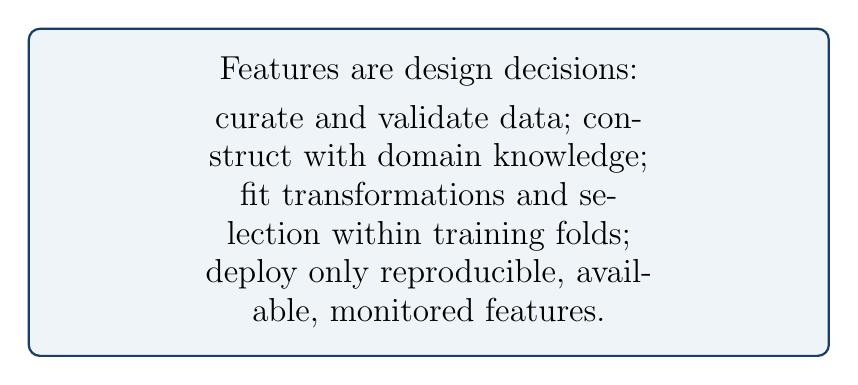
\begin{tikzpicture}
\node[fill=courseice, draw=courseblue, thick, rounded corners=4pt, inner sep=10pt, text width=0.78\textwidth, align=center, font=\large] {Features are design decisions:\\[0.3em] curate and validate data; construct with domain knowledge;\\ fit transformations and selection within training folds;\\ deploy only reproducible, available, monitored features.};
\end{tikzpicture}

\vfill
{\Large\bfseries\color{courseblue} Thank you for your attention.}

\vspace{0.4em}
{\small\color{coursegray} Next: Class 17 --- version control with Git.}
\vfill
\coursefooter
\end{frame}
\end{document}
